\section{Niederschlag}

\subsection{Regenmelder}
\begin{multicols}{2}
{ \centering
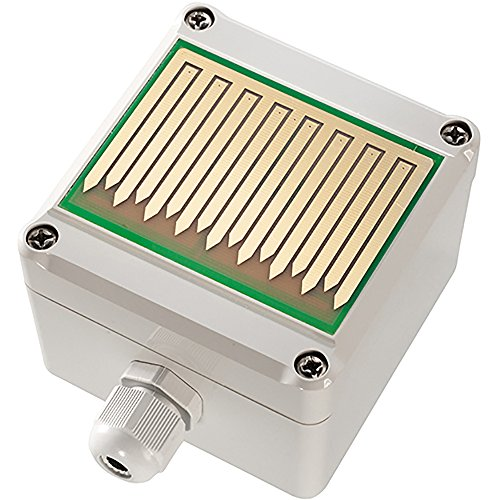
\includegraphics[width=0.4\columnwidth]{graphics/regenmelder.jpg}\\
\captionof{figure}{Regenmelder}
\label{regenmelder}
}
\columnbreak
Es gibt Regenmelder, welche einfach nur den Regen detektieren. Dafür können kapazitive Regensensoren verwendet werden, welche herausfinden ob es regnet oder nicht. Diese müssen seitlich montiert werden, dass das Wasser abläuft und sie müssen zwingend beheizt sein damit der Sensor wieder trocknen kann. \cite[S.51]{Hesse2014} 
\end{multicols}

\subsection{Niederschlagsmesssensor}
Mit diesem Instrument kann der Niederschlag gemessen werden, welcher in einem bestimmten Zeitintervall gefallen ist (Regen, Schnee wenn dieser zu seinem Wasseräquivalent geschmolzen ist und allenfalls Hagel). Dabei gibt es für dieses Projekt verschiedene Verfahren zur Messung, welche in Frage kommen könnten\footnote{wurden direkt priorisiert}:
\begin{itemize}
\item[1.] Disdrometer
\item[2.] Kippwaage
\item[3.] Wägeprinzip
\end{itemize}
\begin{figure}[hbtp]
\centering
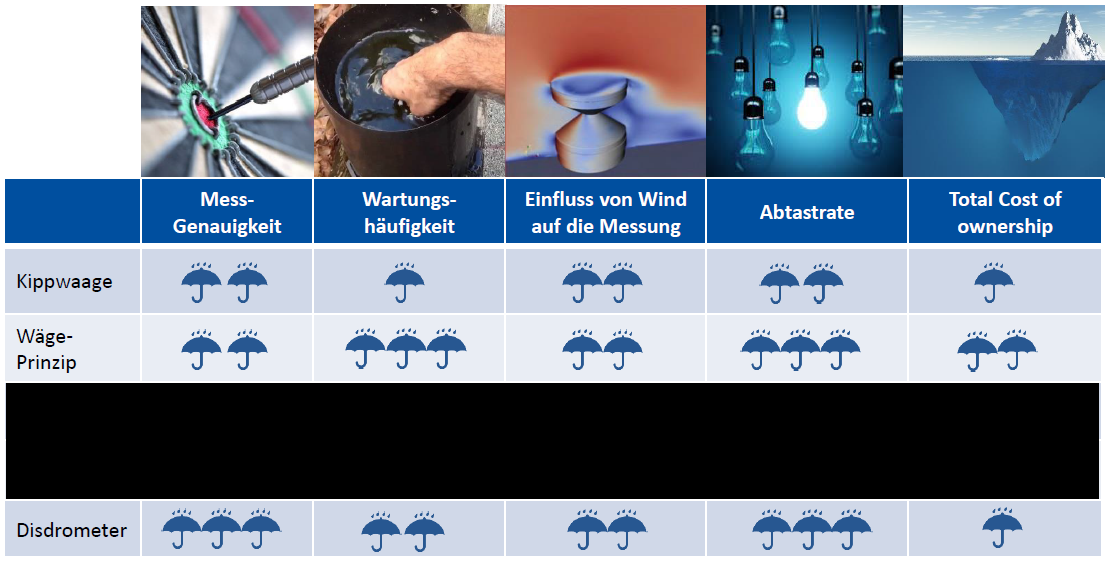
\includegraphics[width=\textwidth]{graphics/vergleich_verfahren.PNG}
\caption{Vergleich der Verfahren}
\label{vergleich_der_verfahren}
\end{figure}

\subsubsection{Disdrometer}
Ein Disdrometer misst im Gegensatz zu den anderen beiden Messverfahren nicht nur die Niederschlagsmenge, sondern auch die Niederschlagsart. Die Messung erfolgt zeit kontinuierlich. Für das Projekt würde also zum Beispiel der \textit{WS100} der Firma Lufft in Frage kommen. Allerdings ist der Preis unbekannt und müsste bei der Firma nachgefragt werden\footnote{Datenblatt der technischen Daten ist im Anhang hinterlegt}.

\subsubsection{Kippwaage}